\maketitle

\begin{abstract}
Simple Linux Utility for Resource Management (SLURM) is an open source,
fault-tolerant, and highly scalable batch system for Linux clusters of 
thousands of nodes.  Components include machine status, partition
management, job management, and scheduling modules.  The design also 
includes a scalable, general-purpose communication infrastructure.
Development will take place in three phases:  Phase I results in a solid
infrastructure;  Phase II produces a functional but limited batch capability
suitable for production deployment; and Phase III addresses the limitations
of Phase III and prepares for open source release in conjunction with 
Livermore's Distributed Production Control System (DPCS), a metabatch and
resource management system.
\end{abstract}

\vspace{0.25in}

\begin{center}

\epsfig{file=slurm.eps,width=4in}
\end{center}

\newpage



\section{Overview}

Our objective is to design and develop an open source Simple Linux Utility for
Resource Management (SLURM) suitable for use on Linux clusters with a few
thousand nodes.  It must be flexible, secure, fault-tolerant and highly
scalable.  Capabilities will include: 

\begin{itemize}
\item Machine and job status: Monitor and record the state of each node in the
cluster. 
\item Partition management: Distinct functionality or capabilities would be
associated with different sets of nodes in the cluster. Each such set of nodes
would be considered a partition. 
\item Switch management: Monitor and manage the node interconnect.
\item Job management: Accept, initiate, delete and otherwise manage the state of
all jobs in the system.
\item Scheduling: Decide when and where to initiate pending jobs.
\end{itemize}

We will strive to complement existing OSCAR work, but replace some of the
existing PBS functionality. Where applicable, we will adhere to existing
standards and reuse existing open source code. No kernel modifications will be
required for basic functionality, although expanded capabilities might be
provided with minor kernel modifications (e.g. gang scheduling). 

\begin{figure}
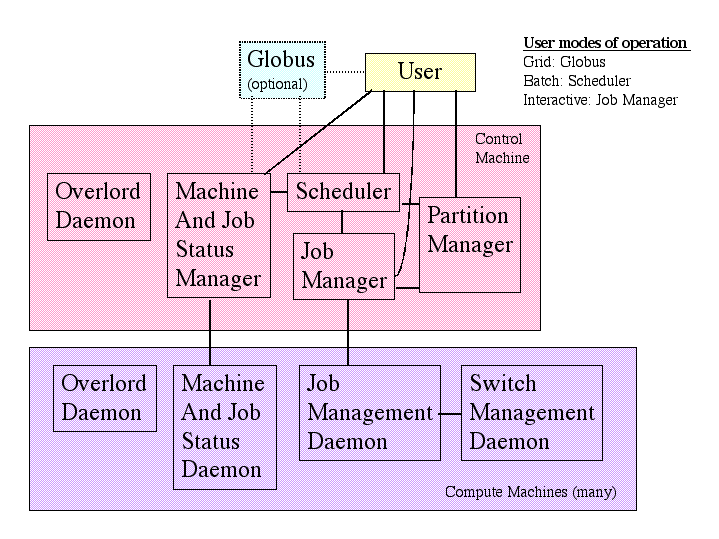
\epsfig{file=LCM.arch.ps,width=6in}
\caption{SLURM Architecture}
\label{arch}
\end{figure}
The design below calls for the designation of a single computer for control of
the cluster with automatic fail-over to a backup computer. A common user home
directory across all nodes of the cluster is assumed. We assume the nodes will
be running the Linux operating system, but will design so as to simplify
support of other operating systems. We assume the nodes will be interconnected
with Quadrics or Gigabit Ethernet, although modular design will simplify
integration of code to support other interconnects. We assume access to this
with Quadrics or Gigabit Ethernet, although modular design will simplify
integration of code to support other interconnects. We assume access to this
interconnect will be restricted to nodes of this cluster for security reasons.
It is desirable that the times on all nodes be synchronized using NTP or other
means, although that will not be required for the SLURM operations. The job's
STDIN, STDOUT, and STDERR will be routed to/from the initiating shell.
Interrelationships between the components are shown in Figure~\ref{arch}
and details of the component follow. 

It should be noted that the architecture is quite similar to that of IBM's
LoadLeveler and Quadrics' RMS; there are only so many ways to manage parallel
machines. This work is distinguished by:
\begin{itemize}
\item Simplicity: The compute machine software component is very light-weight with
the control machine dealing with all concerns about routing work. Most of the
complexity would be in the scheduling component, which could be quite simple if
so desired. Our goal is to provide a solid foundation for cluster management.
\item Scalability: Message traffic will utilize high-fan-out hierarchical
communications with the ability to delegate the confirmation of commands and
collection of acknowledgements (also hierarchical).
\item Open source: We encourage collaborative development.
\end{itemize}

The design below calls for a three-phase development process. Phase one will
develop some of the required cluster management infrastructure: a highly
scalable communications infrastructure, a daemon for utilizing it in a general
fashion, and node status daemons. This infrastructure is expected to be of
great general value for moving data and running programs in a highly scalable
and parallel fashion. There will be no development of a scheduler in phase one.
Phase two will provide basic job management functionality: job, partition and
switch management daemons, but with DPCS' central manager on a distinct (AIX)
computer. Phase three will provide complete job scheduling and management
capabilities including: DPCS' central manager on Linux,.



\section{Machine Status}

Daemons will be required on each node in the cluster to monitor its state.
While existing tools can be combined for machine status and management, such an
emons will be required on each node in the cluster to monitor its state.
While existing tools can be combined for machine status and management, such an
arrangement lacks the scalability required for the support of thousands of
nodes. We believe this poses serious problems in the management of large Linux
clusters and feel compelled to address this issue. 

We recognize the severe impact system daemons can have on performance of
parallel jobs, so the compute and memory resources consumed by this daemon
should be minimized. In phase two, we intend for this service to also monitor
job state and resource consumption by the jobs. Providing these two functions
within a single daemon will minimize system overhead. Information that we
intend to collect on the nodes includes:

\begin{itemize}
\item Count of processors on the node
\item Speed of the processors on the node
\item Size of real memory on the node
\item Size of virtual memory on the node
\item Size of local disk storage
\item State of node (RUN, IDLE, DRAIN, etc.)
\item Cumulative CPU use (by job, kernel and daemons, possibly reporting 
both user and system time independently)
\item Allocated CPU time (recognizes preempted time, by job, kernel and daemons)
\item Real memory demand (by job, kernel and daemons)
\item Virtual Memory Size (by job, kernel and daemons)
\item Local disk storage use (total by all users)
\end{itemize}

This information is readily available through system calls and reading the
process table. DPCS daemons are available to collect the above data. The
communications protocols in those daemon and logic to associate processes with
jobs would require modification.

It is not likely that each node in the cluster could report such information
directly to the control machine without severe scalability constraints. This
could be remedied by using intermediate nodes in a hierarchical fashion to
coalesce the data. These nodes could be ones not designated for parallel job
execution (e.g. login or I/O processing nodes). A status manager will be
required on the control machine to detect and respond to anomalies as well as
maintain the records. This data collection system is similar to that
required on the control machine to detect and respond to anomalies as well as
maintain the records. This data collection system is similar to that
implemented in DPCS. 

\section{Partition Management}

Partition management will be used to identify groups of nodes to be used for
execution of user jobs. Data to be associated with a partition will include:
\begin{itemize}
\item Name and/or ID number
\item Job types permitted (INTERACTIVE and/or BATCH)
\item Maximum execution time (required at least for interactive jobs)
\item Maximum node count (required at least for interactive jobs)
\item List of associated nodes
\item State of partition (UP, DOWN, DRAINING, etc.)
\item Default (YES or NO)
\item List of permitted users (default is "ALL", future)
\item List of users not permitted (default is "NONE", future)
\end{itemize}

It will be possible to alter this data in real-time in order to effect the
scheduling of pending jobs (currently executing jobs would continue). Unlike
other parallel job management systems, we believe this information can be
confined to the SLURM control machine for better scalability. It would be used
by the Job Manager and Machine Status Manager, which exist only on the control
machine. An API to manage the partitions would be developed first, followed by
a simple command-line tool utilizing the API.

\section{Switch Management}

A daemon on each compute node would be responsible for allocating switch
channels and assigning them to user jobs. The switch channels would be
de-allocated upon job termination. If there are ample switch channels and
bandwidth available, it may be desirable for the SLURM daemons to use the
switch directly for communications. This option will be investigated in phase
three. Switch health monitoring tools will also be investigated in phase
thrree.

\section{Scheduling}

We propose that all scheduling decisions be relegated to DPCS. DPCS has
sophisticated and flexible scheduling algorithms that suit our needs well and
provide the scalability required for this application. Most of the resource
sophisticated and flexible scheduling algorithms that suit our needs well and
provide the scalability required for this application. Most of the resource
accounting and some of the job management functions presently within DPCS would
be moved into the proposed SLURM Job Management and Job Status components. 

DPCS will require some modification to operate within this new, richer
environment. The DPCS Central Manager would also require porting to Linux. It
would be simple for other schedulers including PBS, LSF, and Globus to operate
on the SLURM infrastructure, if so desired. 

The DPCS also writes job accounting records to Unix files. Presently, these are
written to a machine with the Sybase database. This data can be accessed via
command-line and web interfaces with Kerberos authentication and authorization.
We are not contemplating making this database software available through SLURM,
but might consider writing this data to an open source database if so desired.

\section{Job Management}

Jobs will be allocated entire nodes. We will support a homogeneous cluster of
nodes in phase two and plan to properly support scheduling of heterogeneous
nodes in phase three. Node sharing will be supported only temporally (e.g.
time-slicing or  gang scheduling). The core functions to be supported include:
\begin{itemize}
\item Initiate job\footnote{There are considerable issues regarding allocation 
of resources (nodes) to jobs and then associating the  allocation to the job 
as well as relinquishing the allocation at job termination that we need to 
discuss. - Bob Wood; Need partition, CPU count, task count, optional node 
list, etc.  - Gregg Hommes}
\item Will job run query (test if "Initiate job" request would succeed)
\item Status job (including node list, memory and CPU use data)
\item Signal job for termination (following DPCS model of explicit application
registration)
\item Terminate job (remove all processes)
\item Preempt job 
\item Resume job
\item Checkpoint/restart job (future)
\item Change node count of running job (could fail if insufficient resources)
\end{itemize}

Since scheduling decisions are being provided by the scheduling component,
there is no concept of submitting a job to be queued. The concept of gang
scheduling, or time-slicing for parallel jobs, is supported by the preempt and
resume functions. Automatic time-sharing of parallel jobs will not be
supported. Explicit node selection will be optionally specified as part of the
resume functions. Automatic time-sharing of parallel jobs will not be
supported. Explicit node selection will be optionally specified as part of the
will job run and initiate job functions. An API for all functions would be
developed initially followed by a  command-line tool utilizing the API. Future
enhancements could include constraining jobs to a specific CPU count or memory
size within a node, which could be used to space-share the node.

System specific scripts can be executed prior to the initiation of a user job
and after the termination of a user job (e.g. prolog and epilog). These scripts
can be used to establish an appropriate environment for the user (e.g. permit
logins, disable logins, terminate "orphan" processes, etc.). 

\section{Infrastructure: Communications Library}

\begin{figure}
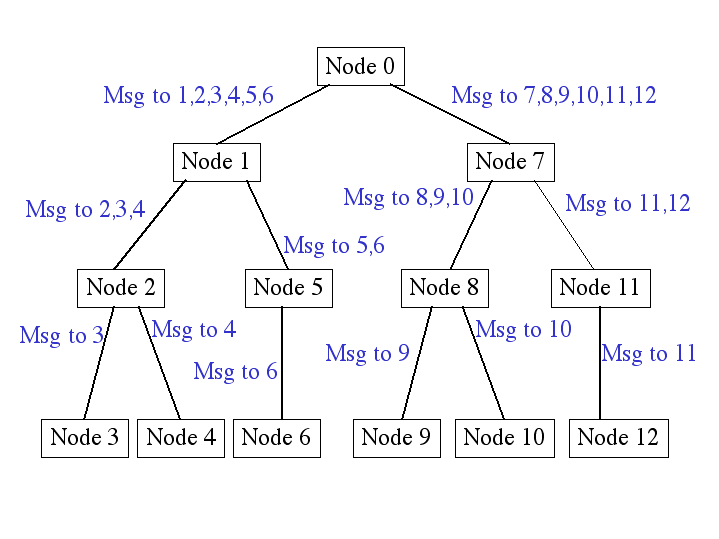
\epsfig{file=LCM.communicate.ps,width=6in}
\caption{Sample communications with fanout = 2}
\label{communicate}
\end{figure}
Optimal communications performance will depend upon hierarchical communications
patterned after DPCS and GangLL work. The SLURM control machine will generate a
list of nodes for each communication. The message will then be sent to one of
the nodes. 
The daemon on that node receiving the message will divide the node list into
two or more new lists of similar size and retransmit the message to one node on
each list. Figure~\ref{communicate} shows the communications for a fan-out of 
two.  Acknowledgements will optionally be sent for the messages to confirm 
receipt with a third message to commit the action. Our design permits the 
control machine to delegate one or more compute machine daemons as responsible 
for fault-tolerance, collection of acknowledgement messages, and the commit
decision. This design minimizes the control machine overhead for performance
reasons. This design also offers excellent scalability and fault 
tolerance.\footnote{Arguments to the communications request include:
\begin{itemize}
\item Request ID
\item Request (command or acknowledgement or commit)
\item List of nodes to be effected
\item Fan-out (count)
\item Commit of request to be required (Yes or No or Delegate node receiving
      message) 
\item Acknowledgement requested to node (name of node or NULL)
\item Acknowledgement requested to port (number)
\end{itemize} }

Security will be provided by the use of reserved ports, which must be opened by
root-level processes. SLURM daemons will open these ports and all user requests
will be processed through those daemons. 

\section{Infrastructure: Other}

We have defined an "overlord" daemon for starting other daemons and insuring
they keep running properly. We will develop configuration management and
logging tools as part of the overload development. These tools will be
they keep running properly. We will develop configuration management and
logging tools as part of the overload development. These tools will be
incorporated into the other daemons. SLURM daemons will have configurable debug
and logging options. The syslog tools will be used for at least some logging
purposes.

The state of control machine daemons will be written periodically both to local
and global file systems to provide fault tolerance. Failures of control machine
daemons will result in their restart by the overlord with state recovery from
disk. If the control machine itself becomes inoperative, its functions can
easily be moved in an automated fashion to another computer. In fact, the
computer designated as alternative control machine can easily be relocated as
the workload on the compute nodes changes. The communications library design is
very important in providing this flexibility.

A single machine will serve as a centralized cluster manager and database. We
do not anticipate user applications executing on this machine. 

\section{Costs}

Very preliminary effort estimates are provided below. More research should
still be performed to investigate the availability of open source code. More
design work is also required to establish more accurate effort estimates.

\begin{center}
\begin{tabular}{|l|c|}\hline
\multicolumn{2}{|c|}{\em I - Basic communication and node status} \\ \hline
Communications Library          & 1.0 FTE month \\
Machine Status Daemon           & 1.5 FTE month \\
Machine Status Manager          & 1.0 FTE month \\
Machine Status Tool             & 0.5 FTE month \\
Overlord Daemon                 & 1.0 FTE month \\
Logging Library                 & 0.5 FTE month \\
{\em TOTAL Phase I}		& {\em 5.5 FTE months} \\ \hline
\multicolumn{2}{|c|}{\em II - Parallel job, switch and partition management} \\ \hline
Basic Switch Daemon             & 2.0 FTE month \\
Job Management Daemon           & 1.0 FTE month \\
Job Manager                     & 2.0 FTE month \\
MPI interface to SLURM          & 2.0 FTE months \\
DPCS uses SLURM Job Manager     & 1.0 FTE months \\
Partition manager               & 2.0 FTE months \\
Switch Health Monitor           & 2.0 FTE months \\
{\em TOTAL Phase II}		& {\em 12.0 FTE months} \\ \hline
\multicolumn{2}{|c|}{\em III - Switch health, and DPCS on Linux} \\ \hline
Job Status Daemon               & 1.5 FTE month \\
DPCS uses SLURM Job Status      & 1.0 FTE months \\
DPCS Controller on Linux        & 0.5 FTE months \\
Fault-tolerant SLURM Managers   & 3.0 FTE months \\
Direct SLURM Switch Use         & 2.0 FTE months \\
{\em TOTAL Phase III}		& {\em 8.0 FTE months} \\ \hline
{\em GRAND TOTAL}		& {\em 25.5 FTE months} \\ \hline
\end{tabular}
\end{center}

\appendix
\newpage

\section{Glossary}

\begin{description}
\item[Condor]	A parallel job manager designed primarily to harness the 
		resources from desktop computers during non-working hours, 
		developed by the University of Wisconsin at Madison
\item[DCE]	Distributed Computing Environment
\item[DFS]	Distributed File System (part of DCE)
\item[DPCS]	Distributed Production Control System, a meta-batch system 
		and resource manager developed by LLNL
\item[GangLL]	Gang Scheduling version of LoadLeveler, a joint development 
		project with IBM and LLNL
\item[Globus]	Grid scheduling infrastructure
\item[Kerberos]	Authentication mechanism
\item[LoadLeveler] IBM's parallel job management system
\item[LLNL]	Lawrence Livermore National Laboratory
\item[NQS]	Network Queuing System (a batch system)
\item[OSCAR]	Open Source Cluster Application Resource
\item[PBS]	Portable Batch System
\item[RMS]	Resource Management System, Quadrics' parallel job management 
		system
\end{description}



\newpage
\section{Review of Related work}

\subsection{PBS (Portable Batch System)}

The Portable Batch System (PBS)\footnote{http://www.openpbs.org/}
is a flexible batch queuing and 
workload management system originally developed by Veridian Systems 
for NASA.  It operates on networked, multi-platform UNIX environments, 
including heterogeneous clusters of workstations, supercomputers, and 
massively parallel systems. PBS was developed as a replacement for 
NQS (Network Queuing System) by many of the same people.

PBS has sophisticated scheduling logic. It spawn's daemons on each 
machine to shepherd the job's tasks (appears to be like LoadLeveler 
and Condor). It provides an interface for administrators to easily 
interface their own scheduling modules (nice feature).  Can support 
long delays in file staging (in and out) with retry.  Host 
authentication provided by checking port number (low ports only 
accessible to root).  Credential service used for user authentication. 
It has the job prolog and epilog feature, which is useful.  Supports 
high priority queue for smaller "interactive" jobs.  Signal to daemons 
causes current log file (e.g. accounting) to be closed, renamed with 
time-stamp, and a new log file created.

Specific complaints about PBS from members of the OSCAR group (Jeremy Enos, 
Jeff Squyres, Tim Mattson):
\begin{itemize}
\item Sensitivity to hostname configuration on the server; improper 
      configuration results in hard to diagnose failure modes.  Once 
      configuration is correct, this issue dissappears.
\item When a compute node in the system dies, everything slows down.  
      PBS is single-threaded and continues to try to contact down nodes,
      while other activities like scheduling jobs, answering qsub/qstat 
      requests, etc., have to wait for a complete timeout cycle before being
      processed.
\item Default schduler is just FIFO, but Maui can be plugged in so this
      is not a big issue.
\item Weak mechanism for starting/cleaning up parallel jobs (pbsdsh).
      When a job is killed, pbsdsh kills the processes it started, but
      if the process doesn't die on the first shot it may continue on.
\item PBS server continues to mark specific nodes offline, even though they 
      are healthy.  Restarting the server fixes this.
\item Lingering jobs.  Jobs assigned to nodes, and then bounced back to the 
      queue for any reason, maintain their assignment to those nodes, even 
      if another job had already started on them.  This is a poor clean up 
      issue.
\item When the PBS server process is restarted, it puts running jobs at risk.
\item Poor diagnostic messages.  This problem can be as serious as ANY other 
      problem.  This problem makes small, simple problems turn into huge 
      turmoil occasionally.  For example, the variety of symptoms that arise 
      from improper hostname configuration.  All the symptoms that result are 
      very misleading to the real problem.
\item Rumored to have problems when the number of jobs in the queues gets
      large.
\item Scalability problems on large systems.
\item Non-portable to Windows
\item Source code is a mess and difficult for others (e.g. the open source
      community) to improve/expand.
\item Licensing problems (see below).
\end{itemize}
The one strength mentioned is PBS's portability and broad user base.

PBS is owned by Veridian and is released as three separate products with
different licenses: {\em PBS Pro} is a commercial product sold by Veridian;
{\em OpenPBS} is an pseudo open source version of PBS that requires 
registration; and
{\em PBS} is a GPL-like, true open source version of PBS.

Bug fixes go into PBS Pro.  When a major revision of PBS Pro comes out,
the previous version of PBS Pro becomes OpenPBS, and the previous version
of OpenPBS becomes PBS.  The delay getting bug fixes (some reported by the
open source community) into the true open source version of PBS is the source
of some frustration.

\subsection{Maui}

Maui Scheduler\footnote{http://mauischeduler.sourceforge.net/}
is an advance reservation HPC batch scheduler for use with SP, 
O2K, and UNIX/Linux clusters. It is widely used to extend the 
functionality of PBS and Loadleveler

\subsection{DPCS}

Something about DPCS here for peer reviewers.

\subsection{LoadLeveler}

LoadLeveler\footnote{
http://www-1.ibm.com/servers/eserver/pseries/software/sp/loadleveler.html}
 is a proprietary batch system and parallel job manager by 
IBM. LoadLeveler supports few non-IBM systems. Very primitive 
scheduling software dependent upon other software for reasonable 
performance (e.g. Maui and DPCS). Many soft and hard limits. Very 
flexible queue and job class structure operating in "matrix" fashion 
(probably overly complex). Many configuration files with signals to 
daemons used to update configuration (like LSF, good). All jobs must 
be initiated through LoadLeveler (no real "interactive" jobs, just 
high priority queue for smaller jobs). Job accounting only available 
on termination (very bad for long-running jobs). Good status 
information on nodes and LSF daemons. Allocates jobs either entire 
nodes or shared nodes depending upon configuration.

A special version of MPI is required. LoadLeveler allocates 
interconnect resources, spawns the user's processes, and manages the 
job afterwards. Daemons also monitor the switch and node health using 
a "heart-beat monitor." One fundamental problem is that when the 
"Central Manager" restarts, it forgets about all nodes and jobs. They 
appear in the database only after checking in via the heartbeat. It 
needs to periodically write state to disk instead of doing 
"cold-starts" after the daemon fails, which is rare. It has the job 
prolog and epilog feature, which permits us to enable/disable logins 
and remove stray processes.

LoadLeveler evolved from Condor, or what was Condor a decade ago. 
While I am less familiar with LSF and Condor than LoadLeveler, they 
all appear very similar with LSF having the far more sophisticated 
scheduler. We should carefully review their data structures and 
daemons before designing our own.

\subsection{LSF (Load Sharing Facility)}


LSF\footnote{http://www.platform.com/}
 is a proprietary batch system and parallel job manager by 
Platform Computing. Widely deployed on a wide variety of computer 
architectures. Sophisticated scheduling software including 
fair-share, backfill, consumable resources, job preemption, many soft 
and hard limits, etc. Very flexible queue structure (perhaps overly 
complex). Most limits are per process rather than per-job (not very 
useful). Time limits include CPU time and wall-clock time. Many 
configuration files with signals to daemons used to update 
configuration (like LoadLeveler, good). All jobs must be initiated 
through LSF (no real "interactive" jobs, just high priority queue for 
smaller jobs). Job accounting only available on termination (very bad 
for long-running jobs). Jobs initiated from same directory as 
submitted from (not good for computer centers with diverse systems 
under LSF control). Good status information on nodes and LSF daemons. 
Allocates jobs either entire nodes or shared nodes depending upon 
configuration.

A special version of MPI is required. LSF allocates interconnect 
resources, spawns the user's processes, and manages the job 
afterwards. While I am less familiar with LSF than LoadLeveler, they 
appear very similar with LSF having the far more sophisticated 
scheduler. We should carefully review their data structures and 
daemons before designing our own.


\subsection{Condor}


Condor\footnote{http://www.cs.wisc.edu/condor/}
 is an open source batch system and parallel job manager 
developed by the University of Wisconsin. Condor was the basis for 
IBM's LoadLeveler and both share very similar underlying 
infrastructure. Condor has a very sophisticated checkpoint/restart 
service that does not rely upon kernel changes, but a variety of 
library changes (which prevent it from being completely general). The 
Condor checkpoint/restart service has been integrated into LSF, 
Codine, and DPCS. Condor is designed to operate across a 
heterogeneous environment, mostly to harness the compute resources of 
workstations and PCs. It has an interesting "advertising" service. 
Servers advertise their available resources and consumers advertise 
their requirements for a broker to perform matches. The checkpoint 
mechanism is used to relocate work on demand (when the "owner" of a 
desktop machine wants to resume work).



\subsection{Memory Channel (Compaq)}

Memory Channel is a high-speed interconnect developed by 
Digital/Compaq with related software for parallel job execution. 
Special version of MPI required. The application spawns tasks on 
other nodes. These tasks connect themselves to the high speed 
interconnect. No system level tool to spawns the tasks, allocates 
interconnect resources, or otherwise manages the parallel job (Note: 
This is sometimes a problem when jobs fail, requiring system 
administrators to release interconnect resources. There are also 
performance problems related to resource sharing).

\subsection{Linux PAGG Process Aggregates}


PAGG\footnote{http://oss.sgi.com/projects/pagg/}
consists of modifications to the linux kernel that allows
developers to implement Process AGGregates as loadable kernel modules.
A process aggregate is defined as a collection of processes that are
all members of the same set. A set would be implemented as a container
for the member processes. For instance, process sessions and groups
could have been implemented as process aggregates.

\subsection{BPROC}


The Beowulf Distributed Process Space 
(BProc\footnote{http://bproc.sourceforge.net/})
is set of kernel
modifications, utilities and libraries which allow a user to start
processes on other machines in a Beowulf-style cluster.  Remote
processes started with this mechanism appear in the process table
of the front end machine in a cluster. This allows remote process
management using the normal UNIX process control facilities. Signals
are transparently forwarded to remote processes and exit status is
received using the usual wait() mechanisms.

\subsection{xcat}

Presumably IBM's suite of cluster management software 
(xcat\footnote{http://publib-b.boulder.ibm.com/Redbooks.nsf/RedbookAbstracts/sg246041.html})
includes a batch system.  Look into this.

\subsection{CPLANT}

CPLANT\footnote{http://www.cs.sandia.gov/cplant/} includes
Parallel Job Launcher, Compute Node Daemon Process,
Compute Node Allocator, Compute Node Status Tool.

\subsection{NQS} 

NQS\footnote{http://umbc7.umbc.edu/nqs/nqsmain.html}, 
the Network Queueing System, is a serial batch system.

\subsection{LAM / MPI}

LAM (Local Area Multicomputer)\footnote{http://www.lam-mpi.org/}
is an MPI programming environment and development system for heterogeneous 
computers on a network. 
With LAM, a dedicated cluster or an existing network
computing infrastructure can act as one parallel computer solving
one problem.  LAM features extensive debugging support in the
application development cycle and peak performance for production
applications. LAM features a full implementation of the MPI
communication standard.

\subsection{MPICH}

MPICH\footnote{http://www-unix.mcs.anl.gov/mpi/mpich/}
is a freely available, portable implementation of MPI,
the Standard for message-passing libraries.

\subsection{Quadrics RMS}

Quadrics
RMS\footnote{http://www.quadrics.com/downloads/documentation/}
(Resource Management System) is a cluster management system for 
Linux and Tru64 which supports the
Elan3 interconnect.  

\subsection{Sun Grid Engine}

SGE\footnote{http://www.sun.com/products-n-solutions/edu/hpc/presentations/june01/omar\_hassaine.pdf}


\subsection{SCIDAC}

The Scientific Discovery through Advanced Computing (SciDAC) 
project\footnote{http://www.scidac.org/ScalableSystems}
has a Resource Management and Accounting working group
and a white paper\cite{Res2000}.

\newpage
\bibliographystyle{plain}
\bibliography{project}
